\documentclass{beamer}

\mode<presentation>
{
  \usetheme{default}
  \usecolortheme{default}
  \usefonttheme{default}
  \setbeamertemplate{navigation symbols}{}
  \setbeamertemplate{caption}[numbered]
  \setbeamertemplate{footline}[page number]
  \setbeamercolor{frametitle}{fg=white}
  \setbeamercolor{footline}{fg=black}
} 

\usepackage[english]{babel}
\usepackage[utf8x]{inputenc}
\usepackage{tikz}
\usepackage{listings}
\usepackage{courier}
\usepackage{array}
\usepackage{bold-extra}
\usepackage{minted}
\usepackage{fancyvrb}

\xdefinecolor{darkblue}{rgb}{0.1,0.1,0.7}
\xdefinecolor{darkgreen}{rgb}{0,0.5,0}
\xdefinecolor{darkgrey}{rgb}{0.35,0.35,0.35}
\xdefinecolor{darkorange}{rgb}{0.8,0.5,0}
\xdefinecolor{darkred}{rgb}{0.7,0,0}
\xdefinecolor{dianablue}{rgb}{0.18,0.24,0.31}
\definecolor{commentgreen}{rgb}{0,0.6,0}
\definecolor{stringmauve}{rgb}{0.58,0,0.82}

\lstset{ %
  backgroundcolor=\color{white},      % choose the background color
  basicstyle=\ttfamily\small,         % size of fonts used for the code
  breaklines=true,                    % automatic line breaking only at whitespace
  captionpos=b,                       % sets the caption-position to bottom
  commentstyle=\color{commentgreen},  % comment style
  escapeinside={\%*}{*)},             % if you want to add LaTeX within your code
  keywordstyle=\color{blue},          % keyword style
  stringstyle=\color{stringmauve},    % string literal style
  showstringspaces=false,
  showlines=true
}

\lstdefinelanguage{scala}{
  morekeywords={abstract,case,catch,class,def,%
    do,else,extends,false,final,finally,%
    for,if,implicit,import,match,mixin,%
    new,null,object,override,package,%
    private,protected,requires,return,sealed,%
    super,this,throw,trait,true,try,%
    type,val,var,while,with,yield},
  otherkeywords={=>,<-,<\%,<:,>:,\#,@},
  sensitive=true,
  morecomment=[l]{//},
  morecomment=[n]{/*}{*/},
  morestring=[b]",
  morestring=[b]',
  morestring=[b]"""
}

\title[2017-04-17-femtocode-diana-implementation]{Femtocode: querying HEP data}
\author{Jim Pivarski}
\institute{Princeton University -- DIANA}
\date{April 17, 2017}

\begin{document}

\logo{\pgfputat{\pgfxy(0.11, 8)}{\pgfbox[right,base]{\tikz{\filldraw[fill=dianablue, draw=none] (0 cm, 0 cm) rectangle (50 cm, 1 cm);}}}\pgfputat{\pgfxy(0.11, -0.6)}{\pgfbox[right,base]{\tikz{\filldraw[fill=dianablue, draw=none] (0 cm, 0 cm) rectangle (50 cm, 1 cm);}
\includegraphics[height=0.99 cm]{diana-hep-logo.png}\tikz{\filldraw[fill=dianablue, draw=none] (0 cm, 0 cm) rectangle (4.9 cm, 1 cm);}}}}

\begin{frame}
  \titlepage
\end{frame}

\logo{\pgfputat{\pgfxy(0.11, 8)}{\pgfbox[right,base]{\tikz{\filldraw[fill=dianablue, draw=none] (0 cm, 0 cm) rectangle (50 cm, 1 cm);}
\includegraphics[height=1 cm]{diana-hep-logo.png}}}}

% Uncomment these lines for an automatically generated outline.
%\begin{frame}{Outline}
%  \tableofcontents
%\end{frame}

%%%%%%%%%%%%%%%%%%%%%%%%%%%%%%%%%%%%%%%%%%%%%%%%%%%%%%%

\begin{frame}{Reminder of motivation}
\vspace{0.3 cm}
\textcolor{gray}{(I last talked about this on December 12.)}

\vfill
\begin{block}{\underline{Query systems}}
In some industries, it is commonplace to query petabytes of data in real time, usually with SQL. (Ibis, Impala, Kudu, Drill, etc.)
\end{block}

\vfill
\uncover<2->{For us, this would mean being able to do final analysis directly on collaboration-shared Analysis Object Datasets (AODs), without managing private skims.}

\vfill
\uncover<3->{However, these systems don't deal (well) with rich objects, like arbitrary-length lists of jets containing lists of tracks.}

\vfill
\begin{uncoverenv}<4->
\begin{block}{\underline{Femtocode}}
I'm developing a query system whose performance permits real-time analysis, but is capable of complex manipulations, such as filtering tracks, picking pairs to compute invariant masses, etc.
\end{block}
\end{uncoverenv}
\end{frame}

\begin{frame}{Three interrelated parts}
\vspace{0.15 cm}
\begin{block}{\underline{Language/compiler}}
\vspace{-0.1 cm}
\begin{itemize}
\item As familiar to the user as possible (objects, nested loops).
\item But constrained to allow restructuring for fast execution (map/filter/reduce instead of for loops, total-functional).
\item Extra-strength type system to eliminate runtime errors.
\end{itemize}
\end{block}

\vspace{-0.2 cm}
\begin{block}{\underline{Execution engine}}
\vspace{-0.1 cm}
\begin{itemize}
\item Operate on contiguous columns of leaf data, rather than objects. Restructuring objects $\to$ changing arrays of integers.
\item No memory allocation at runtime, vectorizable loops.
\item JIT-compiled. CPU target for now, but GPU is possible.
\end{itemize}
\end{block}

\vspace{-0.2 cm}
\begin{block}{\underline{Distributed server}}
\vspace{-0.1 cm}
\begin{itemize}
\item Vending machine: queries go in, histograms (etc.) come out.
\item Referential transparency eliminates the need for ``sessions.''
\end{itemize}
\end{block}
\end{frame}

\begin{frame}[fragile]{Language: working example}
\vspace{0.15 cm}
\scriptsize
\begin{Verbatim}[commandchars=\\\{\}]
pending = session.source(\textcolor{red}{"ZZ_13TeV_pythia8"})
    .define(mumass = \textcolor{red}{"0.105658"})     \textcolor{gray}{# chain of operations on source}
    .toPython(mass = \textcolor{red}{"""}
\textcolor{red}{muons.map(mu1 => muons.map(\{mu2 =>}   \textcolor{gray}{# doubly-nested loop over muons}
\textcolor{red}{  p1x = mu1.pt * cos(mu1.phi);}
\textcolor{red}{  p1y = mu1.pt * sin(mu1.phi);}       \textcolor{gray}{# shares scope with other steps}
\textcolor{red}{  p1z = mu1.pt * sinh(mu1.eta);}      \textcolor{gray}{# in the chain (see "mumass")}
\textcolor{red}{  E1 = sqrt(p1x**2 + p1y**2 + p1z**2 + mumass**2);}

\textcolor{red}{  p2x = mu2.pt * cos(mu2.phi);}
\textcolor{red}{  p2y = mu2.pt * sin(mu2.phi);}
\textcolor{red}{  p2z = mu2.pt * sinh(mu2.eta);}
\textcolor{red}{  E2 = sqrt(p2x**2 + p2y**2 + p2z**2 + mumass**2);}

\textcolor{red}{  px = p1x + p2x; py = p1y + p2y;}
\textcolor{red}{  pz = p1z + p2z; E = E1 + E2;}

\textcolor{gray}{  # "if" is required to avoid sqrt(-x)}
\textcolor{red}{  if E**2 - px**2 - py**2 - pz**2 >= 0:}
\textcolor{red}{    sqrt(E**2 - px**2 - py**2 - pz**2)}
\textcolor{red}{  else:}
\textcolor{red}{    None}   \textcolor{gray}{# output type is nullable}
\textcolor{red}{\}))}
\textcolor{red}{"""}).submit()                        \textcolor{gray}{# asynchronous submission to}
final = pending.await()              \textcolor{gray}{# watch result accumulate}
\end{Verbatim}

\vspace{-4 cm}
\hfill \textcolor{gray}{Yes, we see the Z peak.\hspace{0.25 cm}}

\vspace{-0.2 cm}
\hfill \mbox{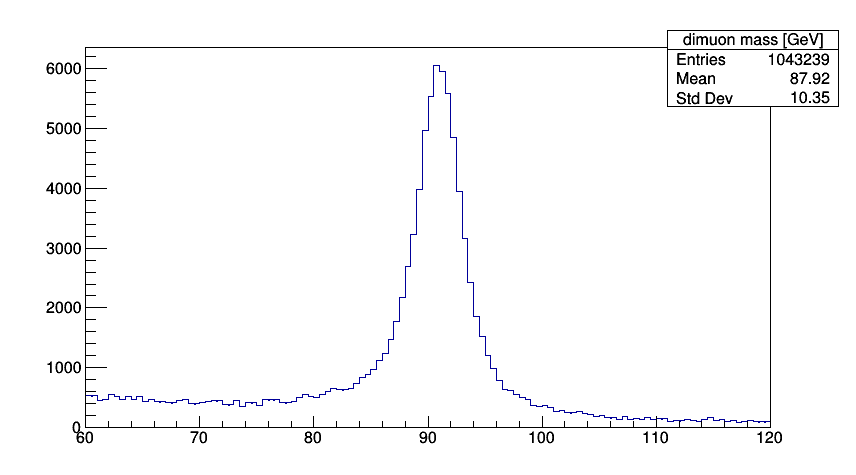
\includegraphics[width=0.48\linewidth]{c1.png}\hspace{-1 cm}}
\vspace{4 cm}

\end{frame}


\end{document}
